% Credit: TeXniCie A-eskwadraat
%
%%% This is a subfile! Type your chapters/section, appendices, etc in here! This code can be run by itself to try for bugs or typo's, but you have to declare your master file for this to work (also references to other files do not work when only compiling this subfile)

% Declare the documentclass. Don't change \documentclass[...]{subfiles}, but replace the ... with the name of your master file.
\documentclass[../main.tex]{subfiles}

% Write the body of the chapter/section/other. You CAN NOT define preamble stuff in here (like \newcommand or \usepackage), that should be done in the preamble.tex instead (which will automatically apply to all subfiles).
\begin{document} % for subfile compilation

\chapter{Local homeomorphisms, sheaf/space adjunction}

\section{Local homeomorphisms}
\remyquote{I don't like annoying stuff, so let's do it the non-annoying way.}
\noindent

\begin{defn}
    A continuous function $f\colon Y\to X$ is said to be a \indexdefnemph{local homeomorphism} if for all $y\in Y$ there exists an open neighbourhood $V_y\subset Y$ such that $f|_{V_y}\colon V_y\to f(V)$ is a homeomorphism onto an open subset of $X$. 
\end{defn}

Later we will see that we may equivalently define an étalé space over $X$ as a topological space $Y$ together with a local homeomorphism $Y\to X$. 
\begin{rmk}
    A local homeomorphism $f\colon Y\to X$ is always open. Namely let $W\subset Y$ be open, then it can be covered by opens of the form $W\cap V_y$, where $f|_{V_y}\colon V_y \to f(V_y)$ are homeomorphisms. Consequently,
\[f(W) = f\bigl(\bigcup_{y\in Y} V_y\cap W \bigr) = \bigcup_{y\in Y} f(V_y\cap W)\text{.}\] Therefore, since $f(V_y\cap W) = f|_{V_y}(V_y\cap W)$ is open in $f(V_y)$, it is open in $X$, thus $f(W)$ is open.
\end{rmk}

\begin{lem}\label{lem:localhomtriangle}
    Let
    \[\begin{tikzcd}[column sep=small]
    Z \arrow[rr, "g"] \arrow[rd, "h"'] &   & Y \arrow[ld, "f"] \\
                                       & X &                  
    \end{tikzcd}\]
    be a commutative triangle in $\catTopologicalSpace$. Then,
    \begin{enumerate}
        \item\label{lem:localhomtriangle:f-g} If $f$ and $g$ are local homeomorphisms then so is $h$.
        \item\label{lem:localhomtriangle:f-h} If $f$ and $h$ are local homeomorphisms then so is $g$.
        \item\label{lem:localhomtriangle:g-open-surj-h} If $g$ is open and surjective and $h$ is a local homeomorphism then so are $f$ and $g$.
    \end{enumerate}
\end{lem}
\begin{proof}
    Argue locally. 
\end{proof}

In particular, by \cref{lem:localhomtriangle:f-g} of the above lemma, we can show that the local homeomorphisms over $X$ form a category $\catLocalHomeomorphism_{/X}$, either as a full subcategory of $\catTopologicalSpace_{/X}$ by \cref{lem:localhomtriangle:f-h}, or as the slice over $X$ of the non-full subcategory $\catLocalHomeomorphism$ of $\catTopologicalSpace$ where all maps are local homeomorphisms.

\begin{exmp} Let $X, Y \in \catTopologicalSpace$ and $U\subset X$ open.
We have the following list of examples:
    \begin{enumerate}
        \item The inclusion $U\hookrightarrow X$ is a local homeomorphism.
        \item Certain covering spaces\index{covering space} $p\colon Y\to X$ are local homeomorphisms.\todo{work out}
        \item Consider the zero locus $V\subset \mathbb{R}^2$ of the polynomial $x-y^3-3y$.
\begin{figure}
    \centering
    \begin{tikzpicture}[scale=0.8]
          \draw[->] (-3, 0) -- (3, 0) node[right] {$x$};
          \draw[->] (0, -3) -- (0, 3) node[above] {$y$};
          \draw[scale=1, domain=-2.1:2.1, smooth, variable=\x] plot ({\x*\x*\x - 3*\x}, {\x});
          % segment around (-2,1)
          \node at (-2,1) {\textbullet};
          \node[scale=0.9] at (-2.7,1) {$(-2,1)$};
          \node[scale=0.8, rotate=22] at (-1.5, 1.384) {$)$};
          \node[scale=0.8, rotate=158] at (-1.5, 0.553) {$($};
          % segment around (2,-1)
          \node at (2,-1) {\textbullet};
          \node[scale=0.9] at (2.7,-1) {$(2,-1)$};
          \node[scale=0.8, rotate=22] at (1.5, -1.384) {$($};
          \node[scale=0.8, rotate=158] at (1.5, -0.553) {$)$};
          % projection and $\mathbb{R}$
          \draw[->] (0,-3.5) -- (0, -4) node at (0.5, -3.75) {$\pr*_x$};
          \draw[<->] (-3, -4.25) -- (3,-4.25) node[right] {$\mathbb{R}$};
          % the images
          \node at (-2, -4.25) {$[$};
          \node at (-1.5, -4.25) {$)$};
          \node[scale=0.8] at (-1.75, -4.75) {}; % {$[-2, -1.5)$};
          \node at (2, -4.25) {$]$};
          \node at (1.5, -4.25) {$($};
          \node[scale=0.8] at (1.75, -4.75) {}; %{$[1.5, 2)$};
    \end{tikzpicture}
    \caption{The projection $\pr*_x\colon V\to \mathbb{R}$ is not a local homeomorphism around the points $(\pm 2,\mp 1)$ since any open neighborhood is projected onto a non-open subset of $\mathbb{R}$.}
    \label{fig:zerolocuslocalhomeo}
\end{figure}
        The projection on the $x$-axis $\pr*_x\colon V \to \mathbb{R}$ is not a local homeomorphism as shown in \cref{fig:zerolocuslocalhomeo}.
        However, after restricting to $V\setminus \{(\pm 2, \mp 1)\}$ it is.
        \item
          Consider the \indexterm{line with two origins} \(\bb R\pushout{\bb R\setminus\{0\}}\bb R\) obtained by gluing two copies of the real line \(\bb R\) along \(\bb R\setminus\{0\}\); see \cref{fig:local-homeomorphisms-line-two-origins}.
          There is a map \(q\) from the disjoint union \(\bb R\cotimes\bb R\) to the line with two origins which sends the origin in the first copy of \(\bb R\) to the one of the two origins in \(\bb R\pushout{\bb R\setminus\{0\}}\bb R\) and the origin in the other copy to the other of the two origins.
          There is a further map \(p\) down to \(\bb R\) which collapses the two origins.
          Both maps \(p\) and \(q\) are local homeomorphisms.

          The line with two origins is not Hausdorff.
          In the second assignment, we will define a sheaf on \(\bb R\) whose étalé space is the line with two origins, illustrating that the étalé space is usually not Hausdorff.
          \begin{figure}
            \centering
            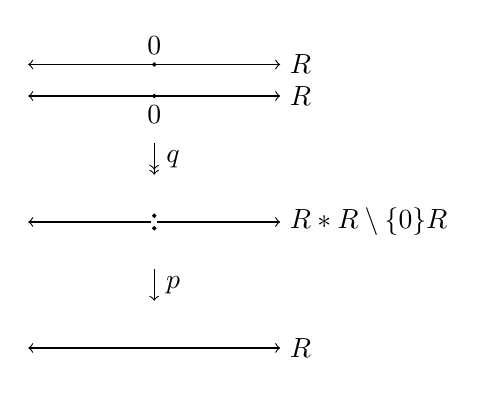
\begin{tikzpicture}[yscale=-1,scale=.8]
              \draw[<->] (-2, 0) -- (2, 0) node[right] {\(\bb R\)};
              \draw[<->] (-2, .5) -- (2, .5) node[right] {\(\bb R\)};
              \draw[fill] (0, 0) circle (0.025) node[above] {\(0\)};
              \draw[fill] (0, .5) circle (0.025) node[below] {\(0\)};
              \draw[->>] (0, 1.25) -- (0, 1.75) node at (0.3, 1.5) {\(q\)};
              \draw[<-] (-2, 2.5) -- (-0.05, 2.5);
              \draw[->] (0.05, 2.5) -- (2, 2.5) node[right] {\(\bb R\pushout*{\bb R\setminus\{0\}}\bb R\)};
              \draw[fill] (0, 2.4) circle (0.025);
              \draw[fill] (0, 2.6) circle (0.025);
              \draw[->] (0, 3.25) -- (0, 3.75) node at (0.3, 3.5) {\(p\)};
              \draw[<->] (-2, 4.5) -- (2, 4.5) node[right] {\(\bb R\)};
            \end{tikzpicture}
            \caption{Two local homeomorphisms related to the line with two origins}
            \label{fig:local-homeomorphisms-line-two-origins}
          \end{figure}
    \end{enumerate}
\end{exmp}

\begin{lem}\label{lem:etalelocalhomeo}
    Let $F$ be a presheaf on \(X\). Then the maps
    \[\coprod_{U\in \open(X)} F(U)\times U \xrightarrow{q} \etalespace(F) \xrightarrow{p} X\]
    are local homeomorphisms, where $q$ is the quotient map and $p\colon [s, x]_U \mapsto x$. 
\end{lem}
\begin{proof}
    \emph{Clearly}, $p\circ q$ is a local homeomorphism. Thus, it suffices to show $q$ is open on opens of the form $(\{s|_V\}\times V)_V$, where $s\in F(U)$, $V\subset U$ opens. For if $q((\{s|_V\}\times V)_V)$ is open, since $(s,x)_U \sim (s|_V,x)_V$ for all $x\in V$, $q((\{s\}\times V)_U) = q((\{s|_V\}\times V)_V)$ is open, so then $q$ is open on all basis opens. Yet since $q$ is a quotient map, this is equivalent to $O:= q^{-1}\circ q((\{s\}\times U)_U)$ being open. So let $(t,x)_V\in O$, then $x\in U$ and $(t,x)_V\sim (s,x)_U$. Hence there exists a $W\subset U\cap V$ such that $t|_W = s|_W$. Thus $(\{t\}\times W)_V \subset F(V)\times V$ is an open neighbourhood of $(t,x)_V$ in $O$. So $q$ is open, therefore, by the previous lemma, $p$ and $q$ are local homeomorphisms.
\end{proof}

Of note, \cref{lem:localhomtriangle:g-open-surj-h} of \cref{lem:localhomtriangle} would not hold if we were to require $g$ to be a quotient map instead of open. As a counterexample, let $I:= [-1,1]\subset \mathbb{R}$. Let $Z = I\cotimes I$ be the disjoint union (with coordinates $(x, \pm 1)$), $Y = Z / \{(\pm 1, -1) \sim (\pm 1, 1)\}\cong S^1$ and $X=I$. Then while $g$ is a quotient map and $h$ a local homeomorphism, $f$ is not a local homeomorphism (in the points $[(\pm 1, 1)]$). 

\section{Sheaf/space adjunction}
\remyquote{Let's go!}
\noindent
We constructed functors
\begin{equation*}
  \begin{tikzcd}
    \catPresheaf(X) \ar[r, "{\etalespace*}"{name=leftadj}, shift left=2] & \catTopologicalSpace_{/X} \ar[l, "h_{-/X}"{name=rightadj}, shift left=2]
  \end{tikzcd}
\end{equation*}
and showed that $\etalespace*$ lands in $\catLocalHomeomorphism_{/X}$ and $h_{-/X}$ lands in $\catSheaf(X)$.

\begin{thm}\label{thm:sheaf-space-adjunction}
There is an adjunction
\begin{equation*}
  \begin{tikzcd}
    \catPresheaf(X) \ar[r, "{\etalespace*}"{name=leftadj}, shift left=2] & \catTopologicalSpace_{/X} \ar[l, "h_{-/X}"{name=rightadj}, shift left=2]
    \ar[from=leftadj, to=rightadj, phantom, "\leftadj" marking]
  \end{tikzcd}
\end{equation*}
which restricts to an adjoint equivalence
\begin{equation*}
  \begin{tikzcd}
    \catSheaf(X) \ar[r, "{\etalespace*}"{name=leftadj}, shift left=2] & \catLocalHomeomorphism_{/X} \ar[l, "h_{-/X}"{name=rightadj}, shift left=2]
    \ar[from=leftadj, to=rightadj, phantom, "\simeq"]
  \end{tikzcd}
\end{equation*}
\end{thm}

\begin{exmp}
Let's check the adjunction for the sheaf $h_{U/X} = h_U = \Hom[\open(X)](-,U)$.
We showed in \cref{exmp:representable-presheaf-espace-étalé} that $\etalespace(h_{U/X}) = U$ in $\catTopologicalSpace_{/X}$.
On the other hand, the Yoneda~\cref{lem:yoneda} gives
\[ \Hom[\catPresheaf(X)](h_U,h_{Y/X}) \cong h_{Y/X}(U) = \cont[X](U,Y)\text{.} \]
Some formal nonsense if you want to feel fancy at dinner parties: $\etalespace*$ is `by definition' the left \indexterm{Kan extension} of
\[ \open(X)\to\catTopologicalSpace_{/X}\text{,} \quad U \mapsto (U\hookrightarrow X) \]
along the Yoneda embedding\index{Yoneda lemma!Yoneda embedding} $h\colon\open(X)\to\catPresheaf(X)$.
\end{exmp}

\begin{proof}[of the adjunction in \cref{thm:sheaf-space-adjunction}]
Since $\etalespace(F)$ is the coequaliser of the diagram
\begin{equation*}
    \begin{tikzcd}
        \coprod_{U\subseteq V} F(V)\times U \ar[r, "a", shift left] \ar[r, "b"', shift right] & \coprod_{U} F(U)\times U
    \end{tikzcd}
\end{equation*}
we have
\[ \cont[X](\etalespace(F),Y) \cong \setpred{f\colon\coprod_U F(U)\times U\to Y}{fa=fb} \]
and likewise
\begin{align*}
    \cont[X]\bigl(\coprod_{U\subseteq X} F(U)\times U,Y\bigr) & \cong \prod_{U\subseteq X} \cont[X](F(U)\times U,Y) \\
    & \cong \prod_{U\subseteq X} \Map(F(U),\cont[X](U,Y)) \\
    & = \prod_{U\subseteq X} \Map(F(U),h_{Y/X}(U))
\end{align*}
and
\[ \cont[X]\bigl(\coprod_{U\subseteq V} F(V)\times U,Y\bigr) \cong \prod_{U\subseteq V}\Map(F(V),h_{Y/X}(U))\text{.} \]
The maps $-\circ a,-\circ b\colon\prod_U\Map(F(U),h_{Y/X}(U))\to\prod_{U\subseteq V}\Map(F(V),h_{Y/X}(U))$ are induced by
\begin{equation*}
    \begin{tikzcd}[row sep=tiny]
        F(U)\times U & F(V)\times U \ar[l, "\incl*^*\times\id"'] \ar[r, "\id\times \incl*"] & F(V)\times V \\
        (s|_U, x) \ar[u, "\in", phantom, marking] & (s,x) \ar[l, mapsto] \ar[r, mapsto] \ar[u, "\in", phantom, marking] & (s,x) \ar[u, "\in", phantom, marking]
    \end{tikzcd}
\end{equation*}
so they are given by
\begin{equation*}
    \begin{tikzcd}[row sep=tiny]
        \Map(F(U),h_{Y/X}(U)) \ar[r] & \Map(F(V),h_{Y/X}(U)) & \Map(F(V),h_{Y/X}) \\
        \alpha_U \ar[u, "\in", phantom, marking] \ar[r, mapsto] & \alpha_U\circ r^F_{UV}\text{,}\ r^{h_{Y/X}}_{UV}\circ\alpha_V \ar[u, "\in", phantom, marking] & \alpha_V \ar[u, "\in", phantom, marking] \ar[l, mapsto]
    \end{tikzcd}
\end{equation*}
for opens $U\subseteq V\subseteq X$.
Hence $f = (\alpha_U)_U \in \prod_U \Map(F(U),h_{Y/X}(U))$ satisfies $fa=fb$ if and only if it is a natural transformation $F\To h_{Y/X}$.
\end{proof}

A fancy comment: we can express $\Hom[\catPresheaf(\cat C)](F,G)$ as an \indexterm{end}
\[ \Hom[\catPresheaf(\cat C)](F,G) \cong \int_{X\in\ob\cat C} \Map(F(X),G(X))\text{.} \]

\begin{rmk}
To check that adjoint functors
\begin{equation*}
  \begin{tikzcd}
    \cat C \ar[r, "{F}"{name=leftadj}, shift left=2] & \cat D \ar[l, "U"{name=rightadj}, shift left=2]
    \ar[from=leftadj, to=rightadj, phantom, "\leftadj" marking]
  \end{tikzcd}
\end{equation*}
are inverse equivalences of categories, you need to check that the \emph{unit} and \emph{counit} are isomorphisms.
The unit is the natural transformation $\eta\colon\id_{\cat C}\To UF$ whose component $\eta_A$ is the transpose of the identity $\id_{FA}\colon FA\to FA$ under the adjunction $F\leftadj U$.
Dually, the counit is the natural transformation $\epsilon\colon FU\To\id_{\cat D}$ whose component $\epsilon_B$ is the transpose of the identity $\id_{UB}\colon UB\to UB$ under the adjunction.
\end{rmk}

\begin{proof}[of the restricted equivalence in \cref{thm:sheaf-space-adjunction}]
Let $\mathcal F$ be a sheaf on $X$.
The unit $\eta_{\mathcal F}\colon \mathcal F\To h_{\etalespace(\mathcal F)/X}$ takes a section $s\in \mathcal F(U)$ to the section to $\etalespace(\mathcal F)\to X$ given by
\begin{equation*}
    \begin{tikzcd}
        \coprod_V \mathcal F(V)\times V \ar[r, "q", epi] & \etalespace(\mathcal F) \ar[r, "p"] & X \\
        & & U \ar[u, inclusion] \ar[lu, dashed, "(\eta_{\mathcal F})_U(s)" description] \ar[llu, bend left=15]
    \end{tikzcd}
\end{equation*}
where the bottom map takes $x\in U$ to $(s,x)_U$.
We need to show that the map
\[ (\eta_{\mathcal F})_U \colon \mathcal F(U) \to \cont[X](U,\etalespace(\mathcal F)) \]
is a bijection.

For injectivity, suppose $(\eta_{\mathcal F})_U(s) = (\eta_{\mathcal F})_U(t)$ for $s,t\in F(U)$.
Then $(s,x)_U\approx(t,x)_U$ for all $x\in U$, so there exists a neighbourhood $W_x\subseteq U$ of $x$ on which $s$ and $t$ agree, that is, $s|_{W_x}=t|_{W_x}$.
The family $(W_x)_{x\in U}$ covers $U$, so gluing gives $s=t$.

For surjectivity, suppose $f\colon U\to\etalespace(\mathcal F)$ is a section.
For any $x\in U$, pick a lift $(s_x,x)_{V_x}\in\coprod_V F(V)\times V$ of $f(x)\in\etalespace(\mathcal F)$ along $q$, and set $W_x\coloneq(\{s_x\}\times V_x)_{V_x}$.
Without loss of generality, we may assume $V_x$ is contained in $U$ (otherwise, intersect \(V_x\) with \(U\)).
We showed in \cref{lem:etalelocalhomeo} that the restricted maps
\[ W_x \xrightarrow[\cong]{q} q(X) \xrightarrow[\cong]{p} V_x \]
are homeomorphisms.
The opens \(U_x\coloneq f\inv(q(W_x))\) cover \(U\) as \(x\) runs through the points of \(U\) and \(f\) lifts to a map
\[ f|_{U_x}\colon U_x\to F(V_x)\times V_x\text{,} \quad (s_x,x)_{V_x} \]
of the form \((\eta_{\mathcal F})_{U_x}(s_x)\).
By injectivity, we get \(s_x|_{U_x\cap U_y}=s_y|_{U_x\cap U_y}\) for all \(x\) and \(y\), so they glue to a section \(s\in\mathcal F(U)\) such that \(f=(\eta_{\mathcal F})_U(s)\).

We conclude that the unit is an isomorphism for sheaves.
We finish the proof next week by showing that the counit is an isomorphism for local homeomorphisms.
\end{proof}

\end{document} % for the subfile compilation